\documentclass{standalone}
\usepackage{tikz}\usetikzlibrary{shapes,arrows.meta}
\begin{document}
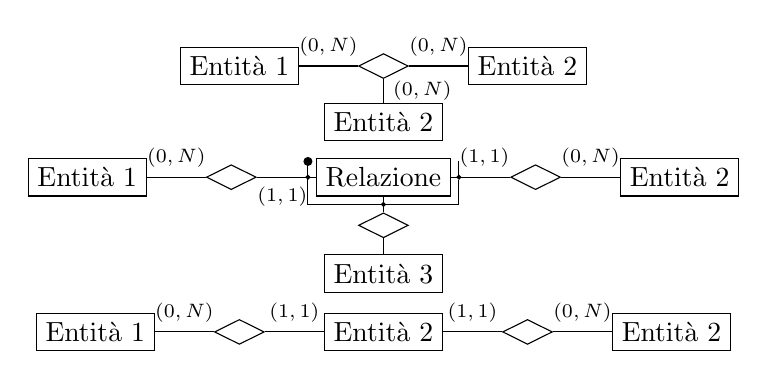
\begin{tikzpicture}
    \draw

    %%* Attributi:
    %%  node[draw, circle, inner sep=1pt, fill=black]{}node[right]{\footnotesize A}
    %%? Distanza orizzontale: E -(0.25,0.x)- A
    %%? Distanza verticale: E -(0,x * 0.22)- A

    %%* Cardinalità:
    %%  node[below right]{\scriptsize $(0,N)$}
    %%  node[above right]{\scriptsize $(0,N)$}
    %%  node[midway, above]{\scriptsize $(0,N)$}

    %%* Relazione:
    %%  node[draw, diamond, shape aspect=2, inner sep=3pt, anchor=90](r1){}
    %%  node[draw, diamond, shape aspect=2, inner sep=0.2pt, anchor=180](r2){R2}

    %%* Entità:
    %%  node[draw, rectangle, anchor=90](e1){}
    %%? Distanza verticale: E -(0.3)- R -(0.3) E
    %%? Distanza orizzontale: E -(0.75)- R -(0.75)- E

    (0,0)node[draw, rectangle, anchor=90](e1){Entità 1}
    (e1.0)--++(0.75,0)node[midway, above]{\scriptsize $(0,N)$}node[draw, diamond, shape aspect=2, inner sep=3pt, anchor=180](r1){}
    (r1.0)--++(0.75,0)node[midway, above]{\scriptsize $(0,N)$}node[draw, rectangle, anchor=180](e1){Entità 2}
    (r1.270)--++(0,-0.3)node[midway, right]{\scriptsize $(0,N)$}node[draw, rectangle, anchor=90](e1){Entità 2}

    (r1.270)++(0,-1)node[draw, rectangle, anchor=90](e1){Relazione}
    (e1.180)--++(-0.1,0)node[draw, circle, inner sep=0.5pt, fill=black](a){}--++(-.65,0)node[midway, below]{\scriptsize $(1,1)$}node[draw, diamond, shape aspect=2, inner sep=3pt, anchor=0](r1){}
    (r1.180)--++(-.75,0)node[midway, above]{\scriptsize $(0,N)$}node[draw, rectangle, anchor=0](e2){Entità 1}
    (e1.0)--++(0.1,0)node[draw, circle, inner sep=0.5pt, fill=black](b){}--++(.65,0)node[midway, above]{\scriptsize $(1,1)$}node[draw, diamond, shape aspect=2, inner sep=3pt, anchor=180](r1){}
    (r1.0)--++(.75,0)node[midway, above]{\scriptsize $(0,N)$}node[draw, rectangle, anchor=180](e3){Entità 2}
    (e1.270)--++(0,-0.1)node[draw, circle, inner sep=0.5pt, fill=black](c){}--++(0,-0.1)node[draw, diamond, shape aspect=2, inner sep=3pt, anchor=90](r1){}
    (r1.270)--++(0,-0.2)node[draw, rectangle, anchor=90](e4){Entità 3}
    (a)++(0,0.2)node[draw, circle, inner sep=1pt, fill=black]{}|-(c)-|(b)--++(0,0.2)

    (e4.270)++(0,-0.25)node[draw, rectangle, anchor=90](e1){Entità 2}
    (e1.180)--++(-.75,0)node[midway, above]{\scriptsize $(1,1)$}node[draw, diamond, shape aspect=2, inner sep=3pt, anchor=0](r1){}
    (r1.180)--++(-.75,0)node[midway, above]{\scriptsize $(0,N)$}node[draw, rectangle, anchor=0](e2){Entità 1}
    (e1.0)--++(.75,0)node[midway, above]{\scriptsize $(1,1)$}node[draw, diamond, shape aspect=2, inner sep=3pt, anchor=180](r1){}
    (r1.0)--++(.75,0)node[midway, above]{\scriptsize $(0,N)$}node[draw, rectangle, anchor=180](e3){Entità 2}

    ;
\end{tikzpicture}
\end{document}